% This must be in the first 5 lines to tell arXiv to use pdfLaTeX, which is strongly recommended.
\pdfoutput=1
% In particular, the hyperref package requires pdfLaTeX in order to break URLs across lines.

\documentclass[11pt]{article}

\usepackage[review]{acl}

% Standard package includes
\usepackage{times}
\usepackage{latexsym}
\usepackage{amsmath}
\usepackage{graphicx}
\usepackage{booktabs}
\usepackage{amssymb}
\usepackage{hyperref}
\usepackage{float}
\usepackage{tikz}
\usepackage{subcaption} % for subfigures

% For proper rendering and hyphenation of words containing Latin characters (including in bib files)
\usepackage[T1]{fontenc}
% For Vietnamese characters
% \usepackage[T5]{fontenc}
% See https://www.latex-project.org/help/documentation/encguide.pdf for other character sets

% This assumes your files are encoded as UTF8
\usepackage[utf8]{inputenc}

% This is not strictly necessary, and may be commented out.
% However, it will improve the layout of the manuscript,
% and will typically save some space.
\usepackage{microtype}

% This is also not strictly necessary, and may be commented out.
% However, it will improve the aesthetics of text in
% the typewriter font.
\usepackage{inconsolata}


% If the title and author information does not fit in the area allocated, uncomment the following
%
%\setlength\titlebox{<dim>}
%
% and set <dim> to something 5cm or larger.

\title{CSC401 Homework Assignment \#2\\Analysis}

\author{Zixuan Zeng \\
  Student number: \texttt{1008533419} \\
  UTORid: \texttt{zengzix2} \\
  \texttt{zixuan.zeng@mail.utoronto.ca}}

\begin{document}
\maketitle

\section{Training Results}


\paragraph{Response}
{\it Yes, there is a difference between BLEU-3 and BLEU-4. BLEU-3 is slightly higher than BLEU-4, 
because BLEU-3 considers 3-grams of a sentence while BLEU-4 considers 4-grams. 
As n get larger, n-grams are less likely to match up. i.e. 3-grams of candidate is more likely to be present in reference than 4-grams.}

\subsection{Training Loop Printout}

\subsubsection{Model with Pre-layer Normalization}

\begin{figure}[H]
  \centering
  \begin{subfigure}[b]{0.49\textwidth}
    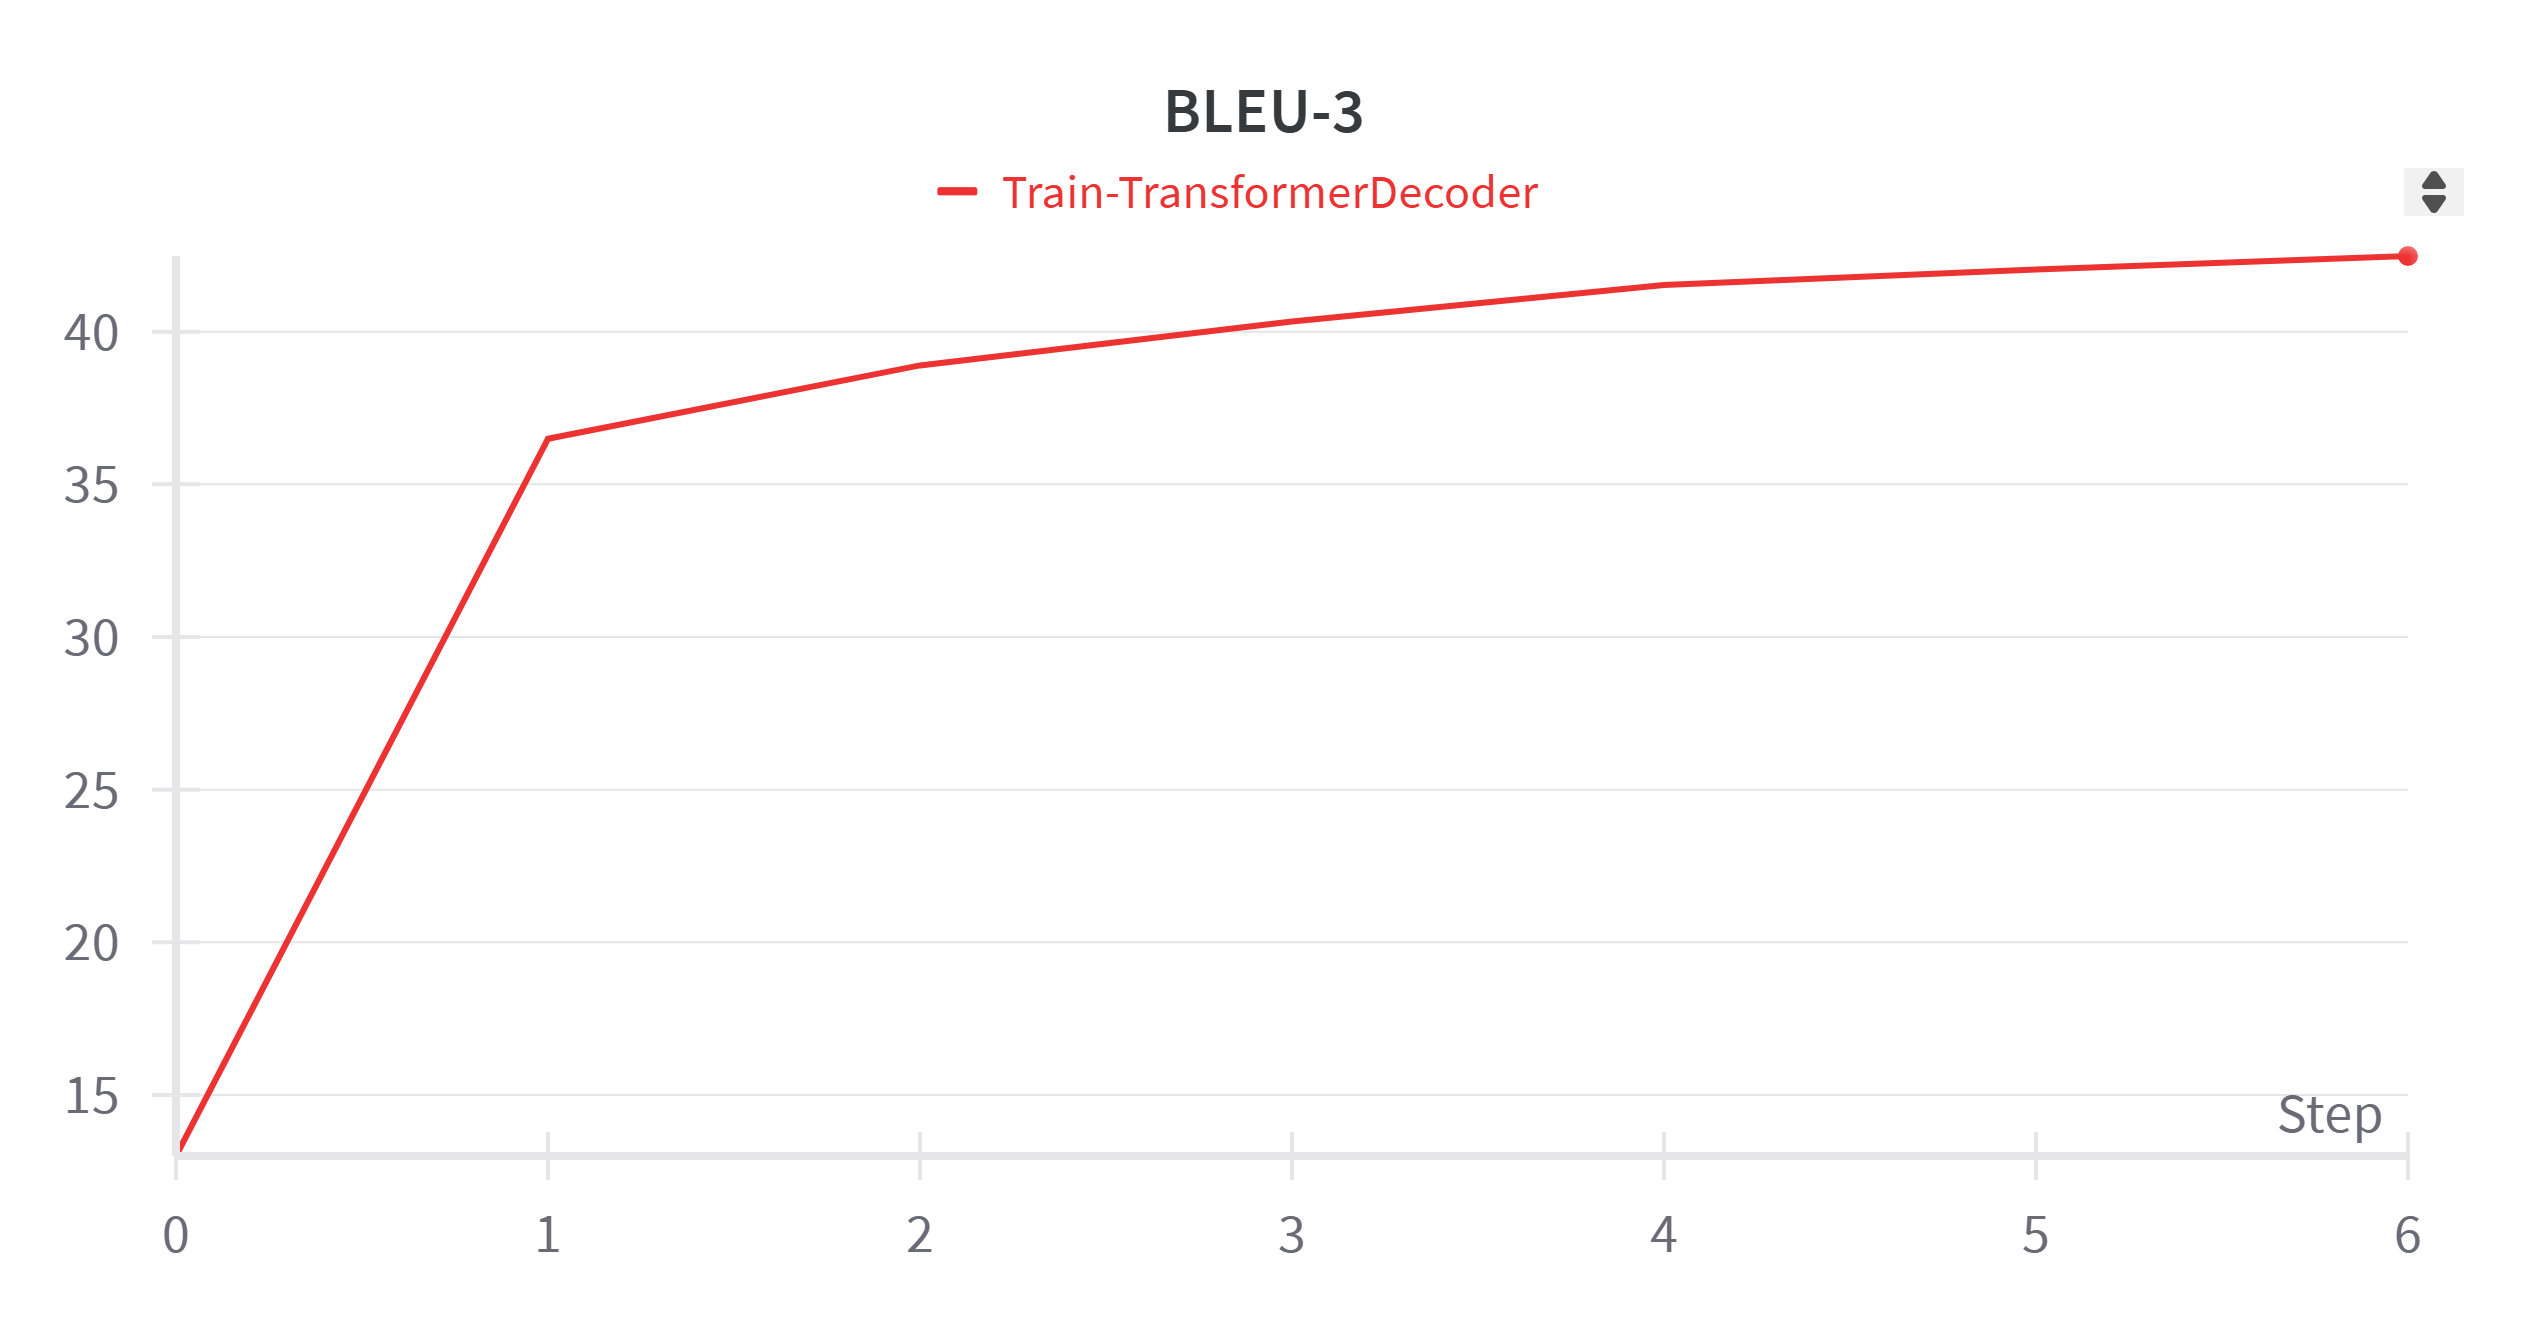
\includegraphics[width=\linewidth]{./wb-pre-bleu3.png}
    \caption{BLEU-3}
    \label{fig:train_bleu_wo_attention}
  \end{subfigure}
  \hfill
  \begin{subfigure}[b]{0.49\textwidth}
    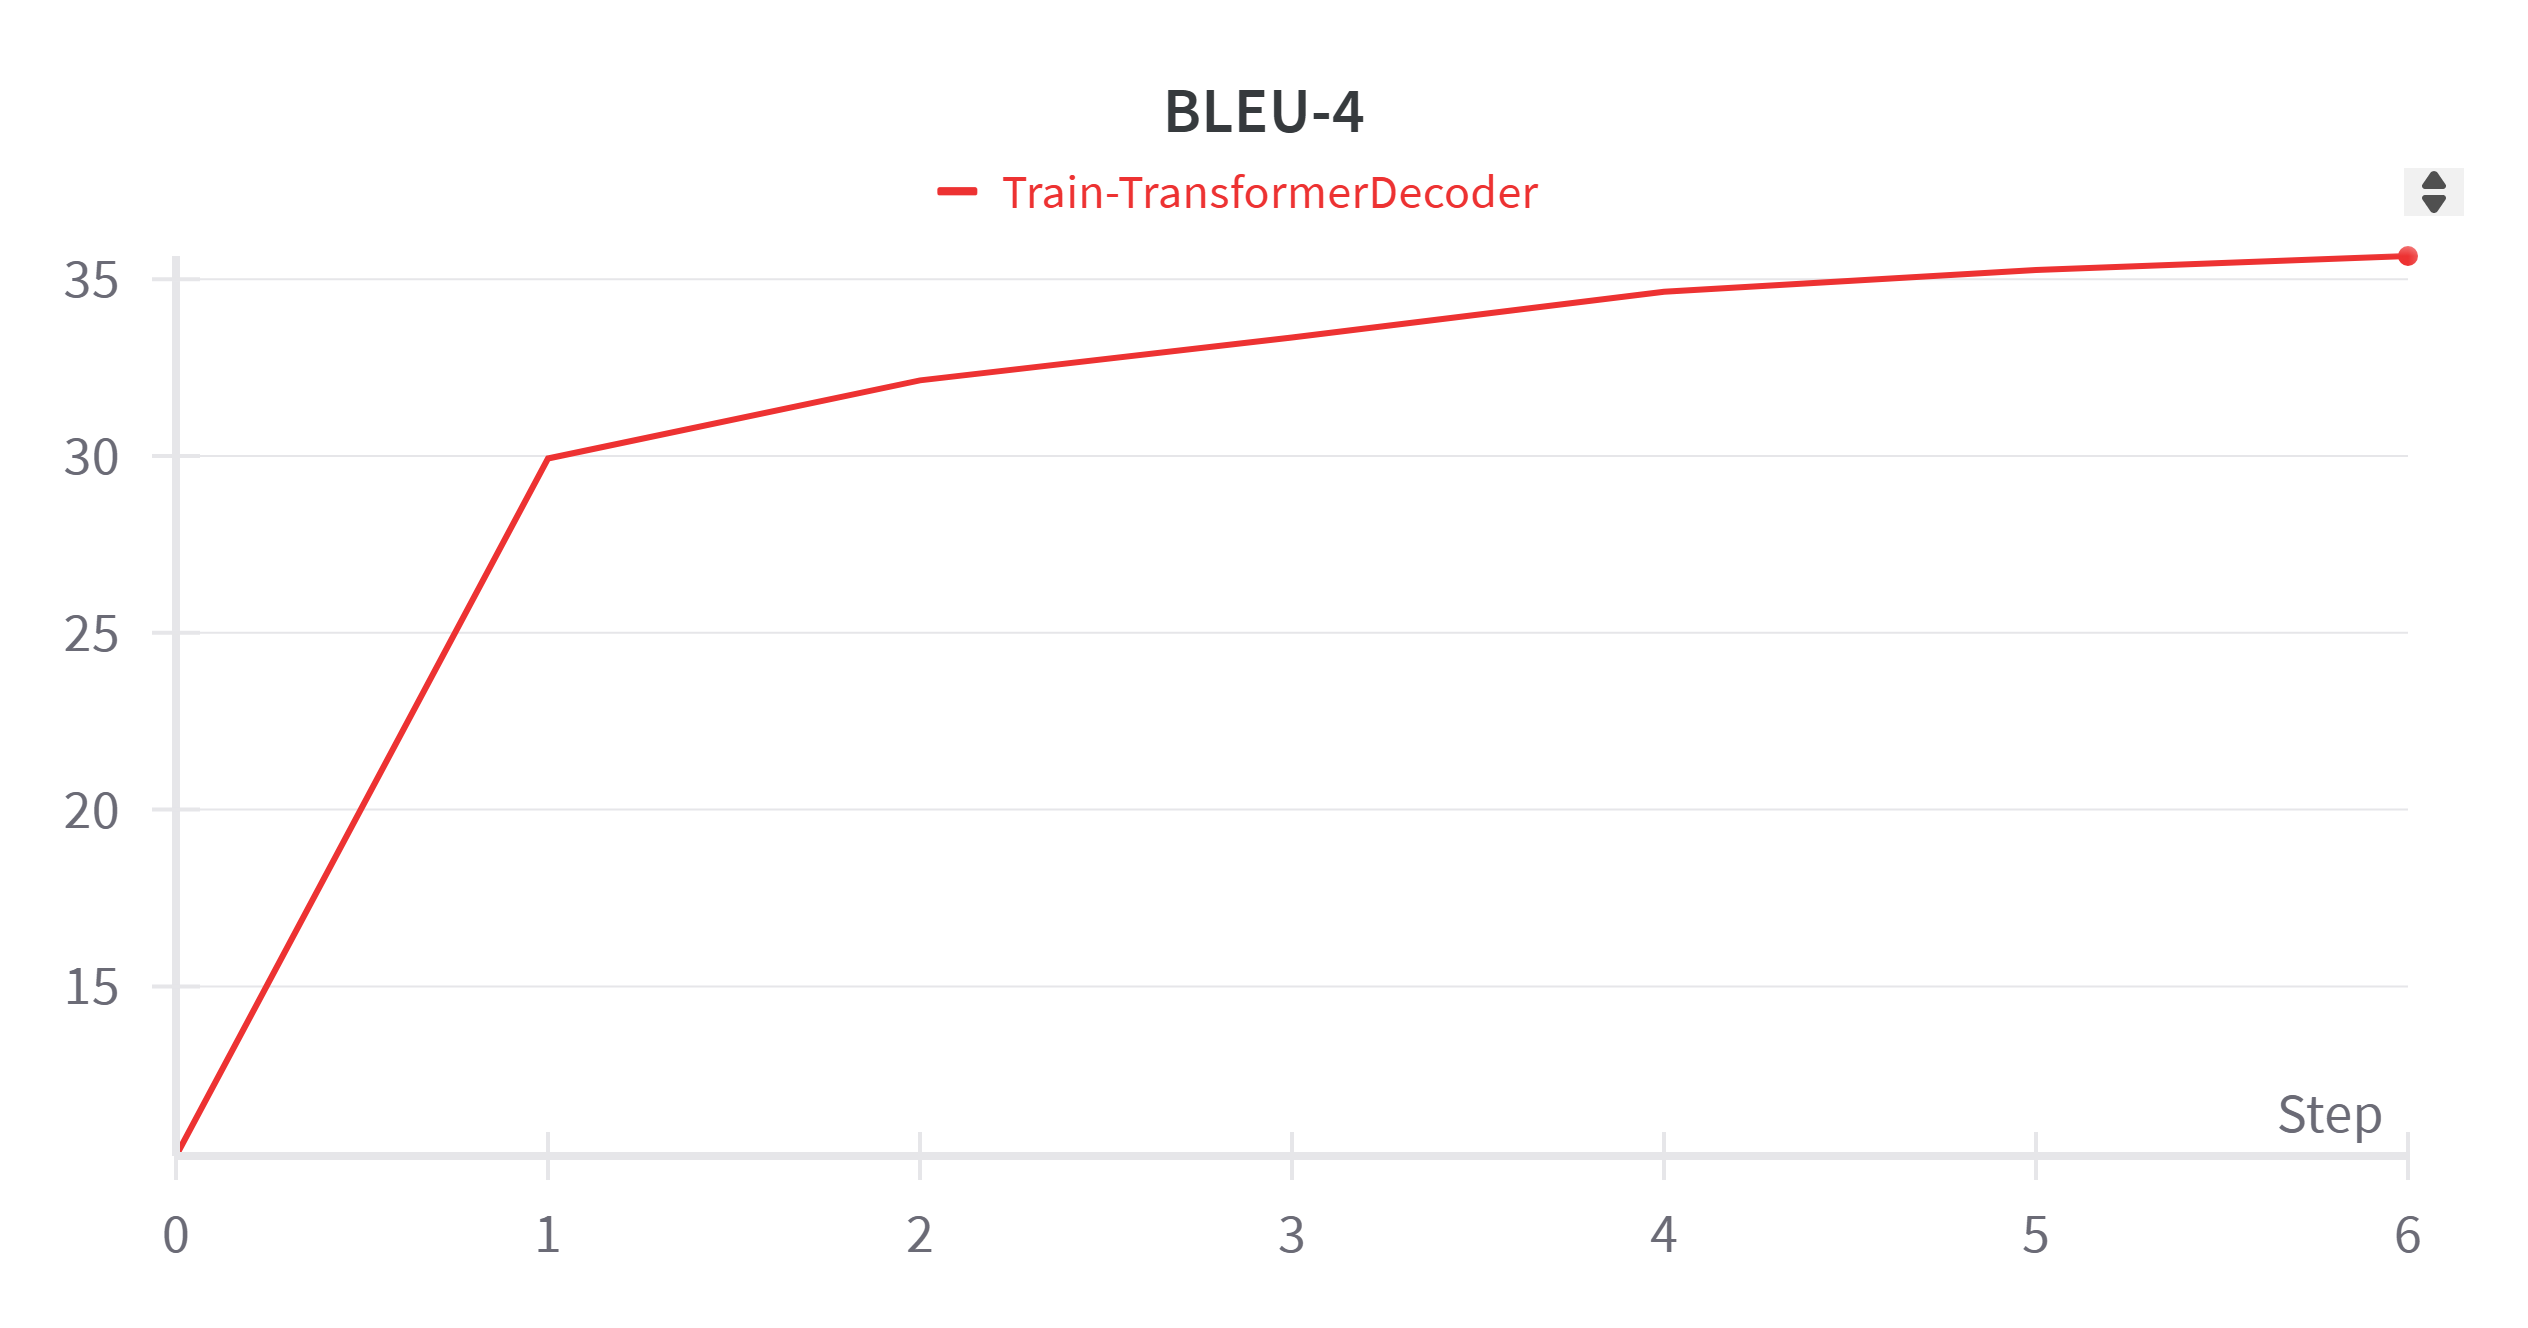
\includegraphics[width=\linewidth]{./wb-pre-bleu4.png}
    \caption{BLEU-4}
    \label{fig:train_bleu_wo_attention}
  \end{subfigure}
  \caption{Wandb Training BLEU Score for Model with Pre-layer Normalization}
  \label{fig:overall}
\end{figure}

\begin{figure}[H]
  \centering
  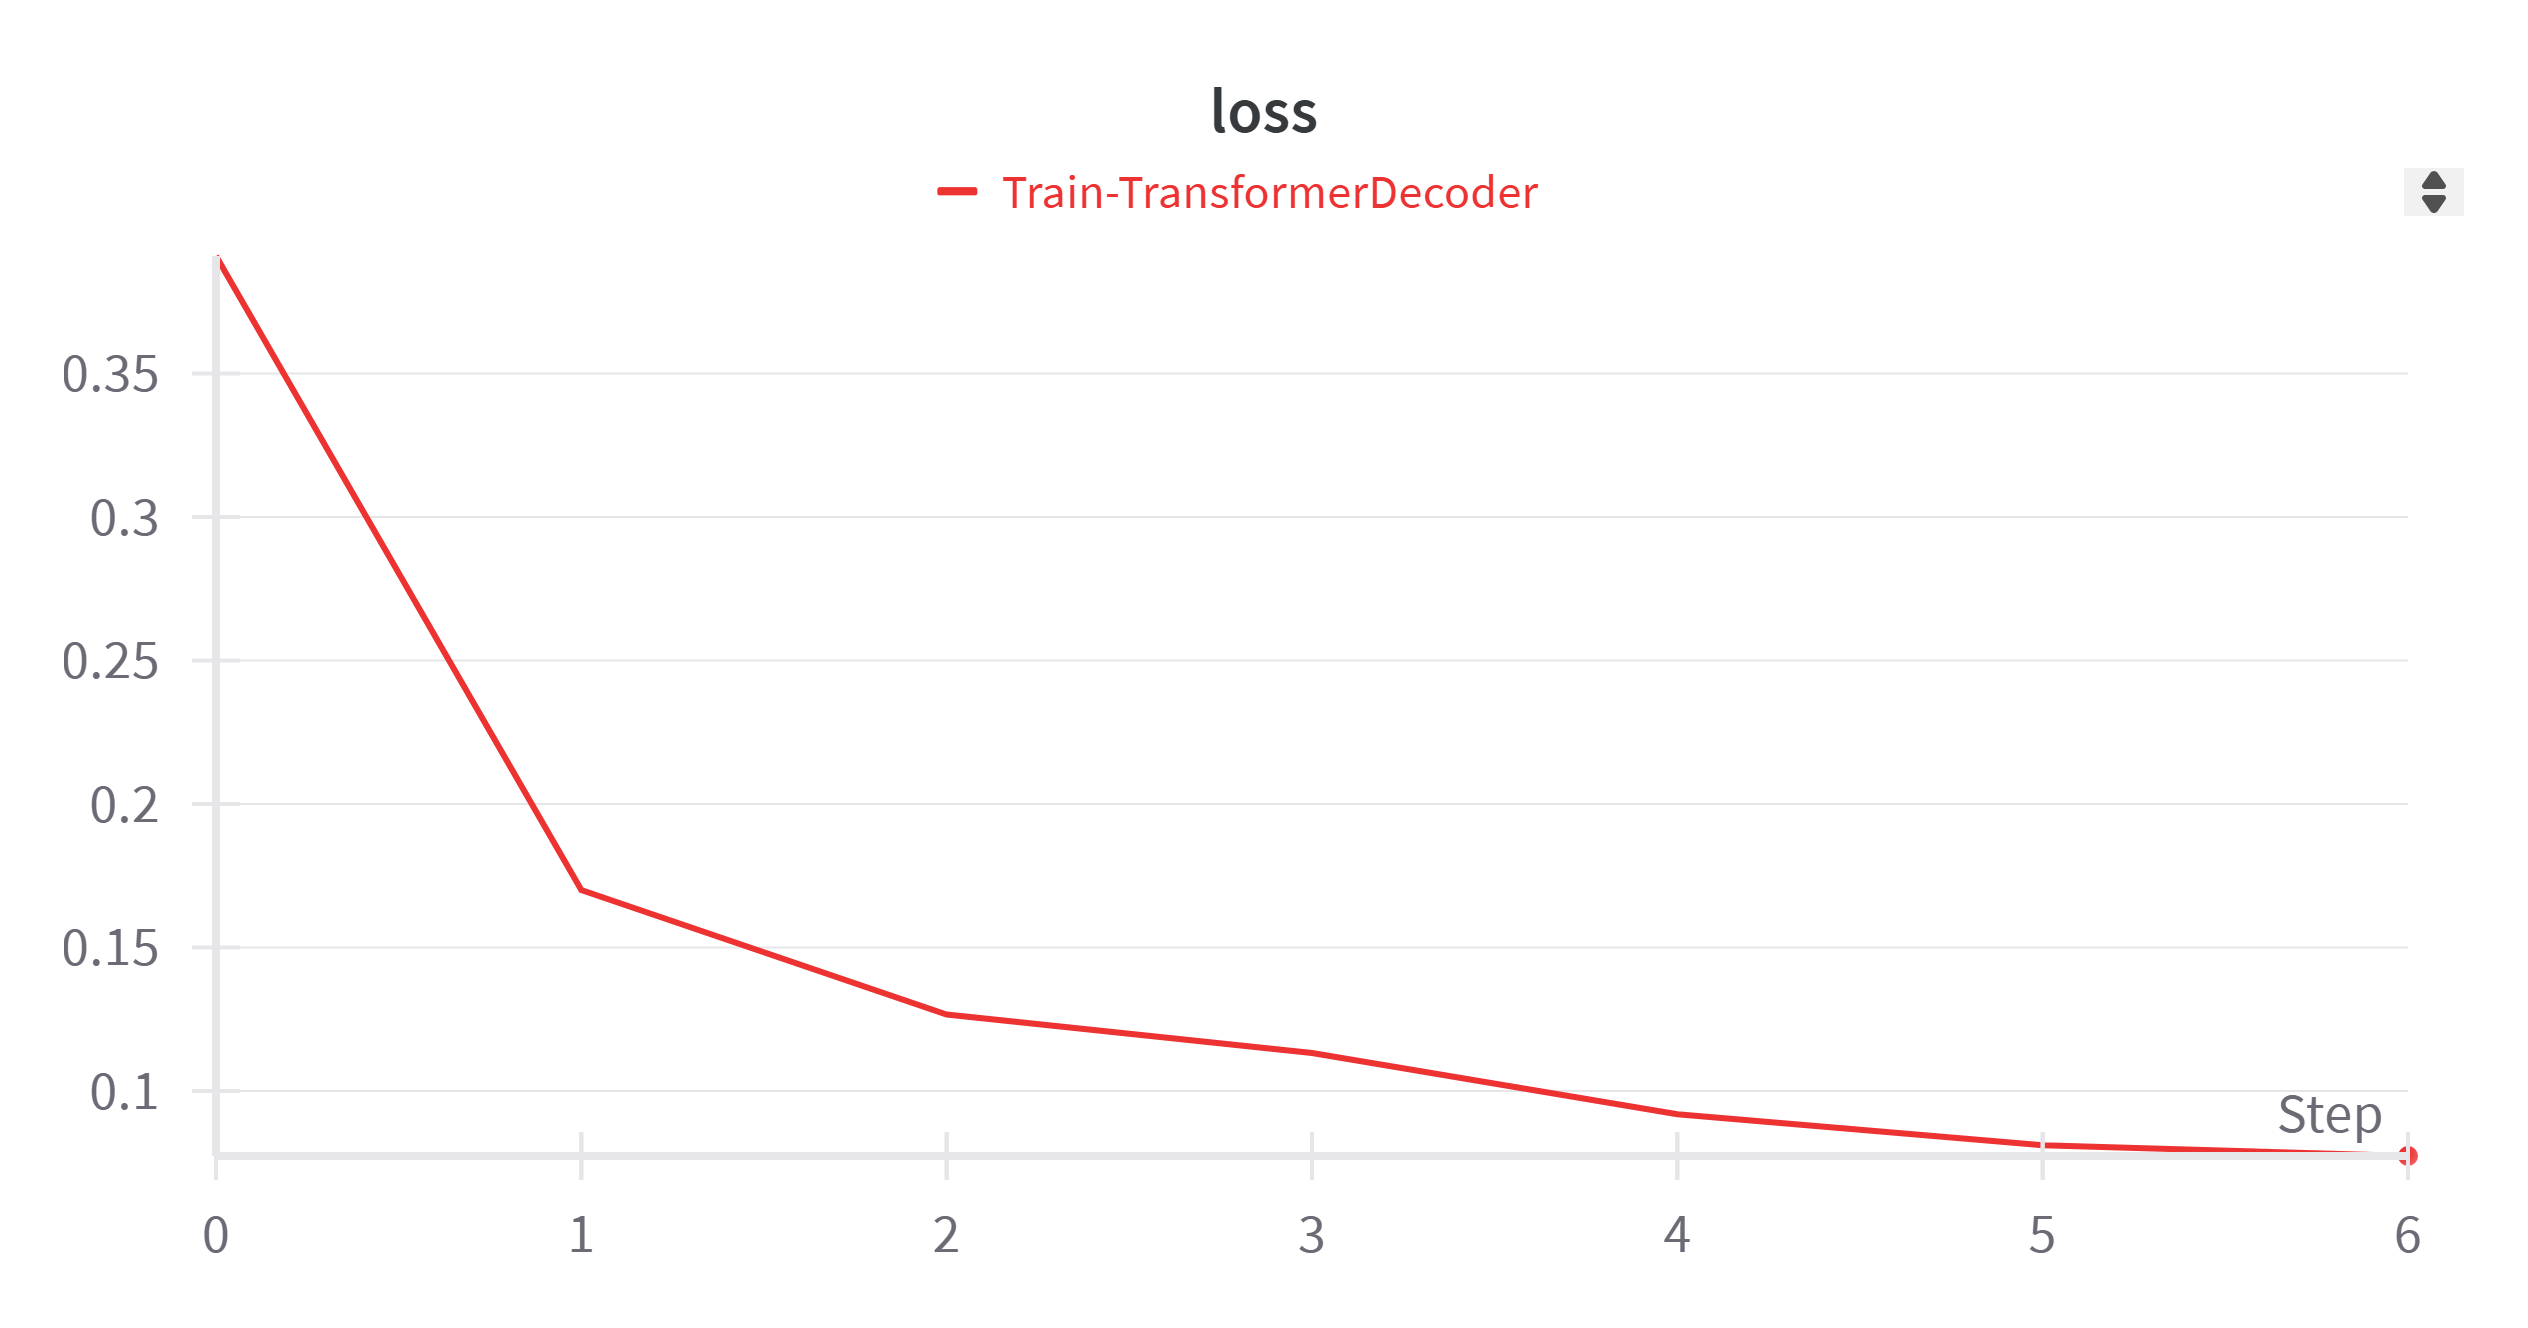
\includegraphics[width=0.5\linewidth]{./wb-pre-loss.png}
  \caption{Wandb Training Loss for Model with Pre-layer Normalization}
  \label{fig:train_loss_wo_attention}
\end{figure}

\begin{small}
\begin{verbatim}
  [Device:cuda] Epoch 1 Training ====
  [Device:cuda] Epoch 1 Validation ====
  Epoch 1: loss=0.3908990512516098, BLEU-4: 10.2027 BLEU-3: 12.9993, time=00:01:57
  [Device:cuda] Epoch 2 Training ====
  [Device:cuda] Epoch 2 Validation ====
  Epoch 2: loss=0.16999544792528534, BLEU-4: 29.9309 BLEU-3: 36.4932, time=00:03:58
  [Device:cuda] Epoch 3 Training ====
  [Device:cuda] Epoch 3 Validation ====
  Epoch 3: loss=0.12660633221681297, BLEU-4: 32.1398 BLEU-3: 38.8967, time=00:05:59
  [Device:cuda] Epoch 4 Training ====
  [Device:cuda] Epoch 4 Validation ====
  Epoch 4: loss=0.11323737249162294, BLEU-4: 33.3536 BLEU-3: 40.3332, time=00:08:00
  [Device:cuda] Epoch 5 Training ====
  [Device:cuda] Epoch 5 Validation ====
  Epoch 5: loss=0.09187625667094113, BLEU-4: 34.6483 BLEU-3: 41.5310, time=00:09:59
  [Device:cuda] Epoch 6 Training ====
  [Device:cuda] Epoch 6 Validation ====
  Epoch 6: loss=0.08105527142436564, BLEU-4: 35.2590 BLEU-3: 42.0404, time=00:11:58
  [Device:cuda] Epoch 7 Training ====
  [Device:cuda] Epoch 7 Validation ====
  Epoch 7: loss=0.07732721824508375, BLEU-4: 35.6572 BLEU-3: 42.4802, time=00:13:59
  Finished 7 epochs
\end{verbatim}
\end{small}

\subsubsection{Model with Post-layer Normalization}
\begin{figure}[H]
  \centering
  \begin{subfigure}[b]{0.49\textwidth}
    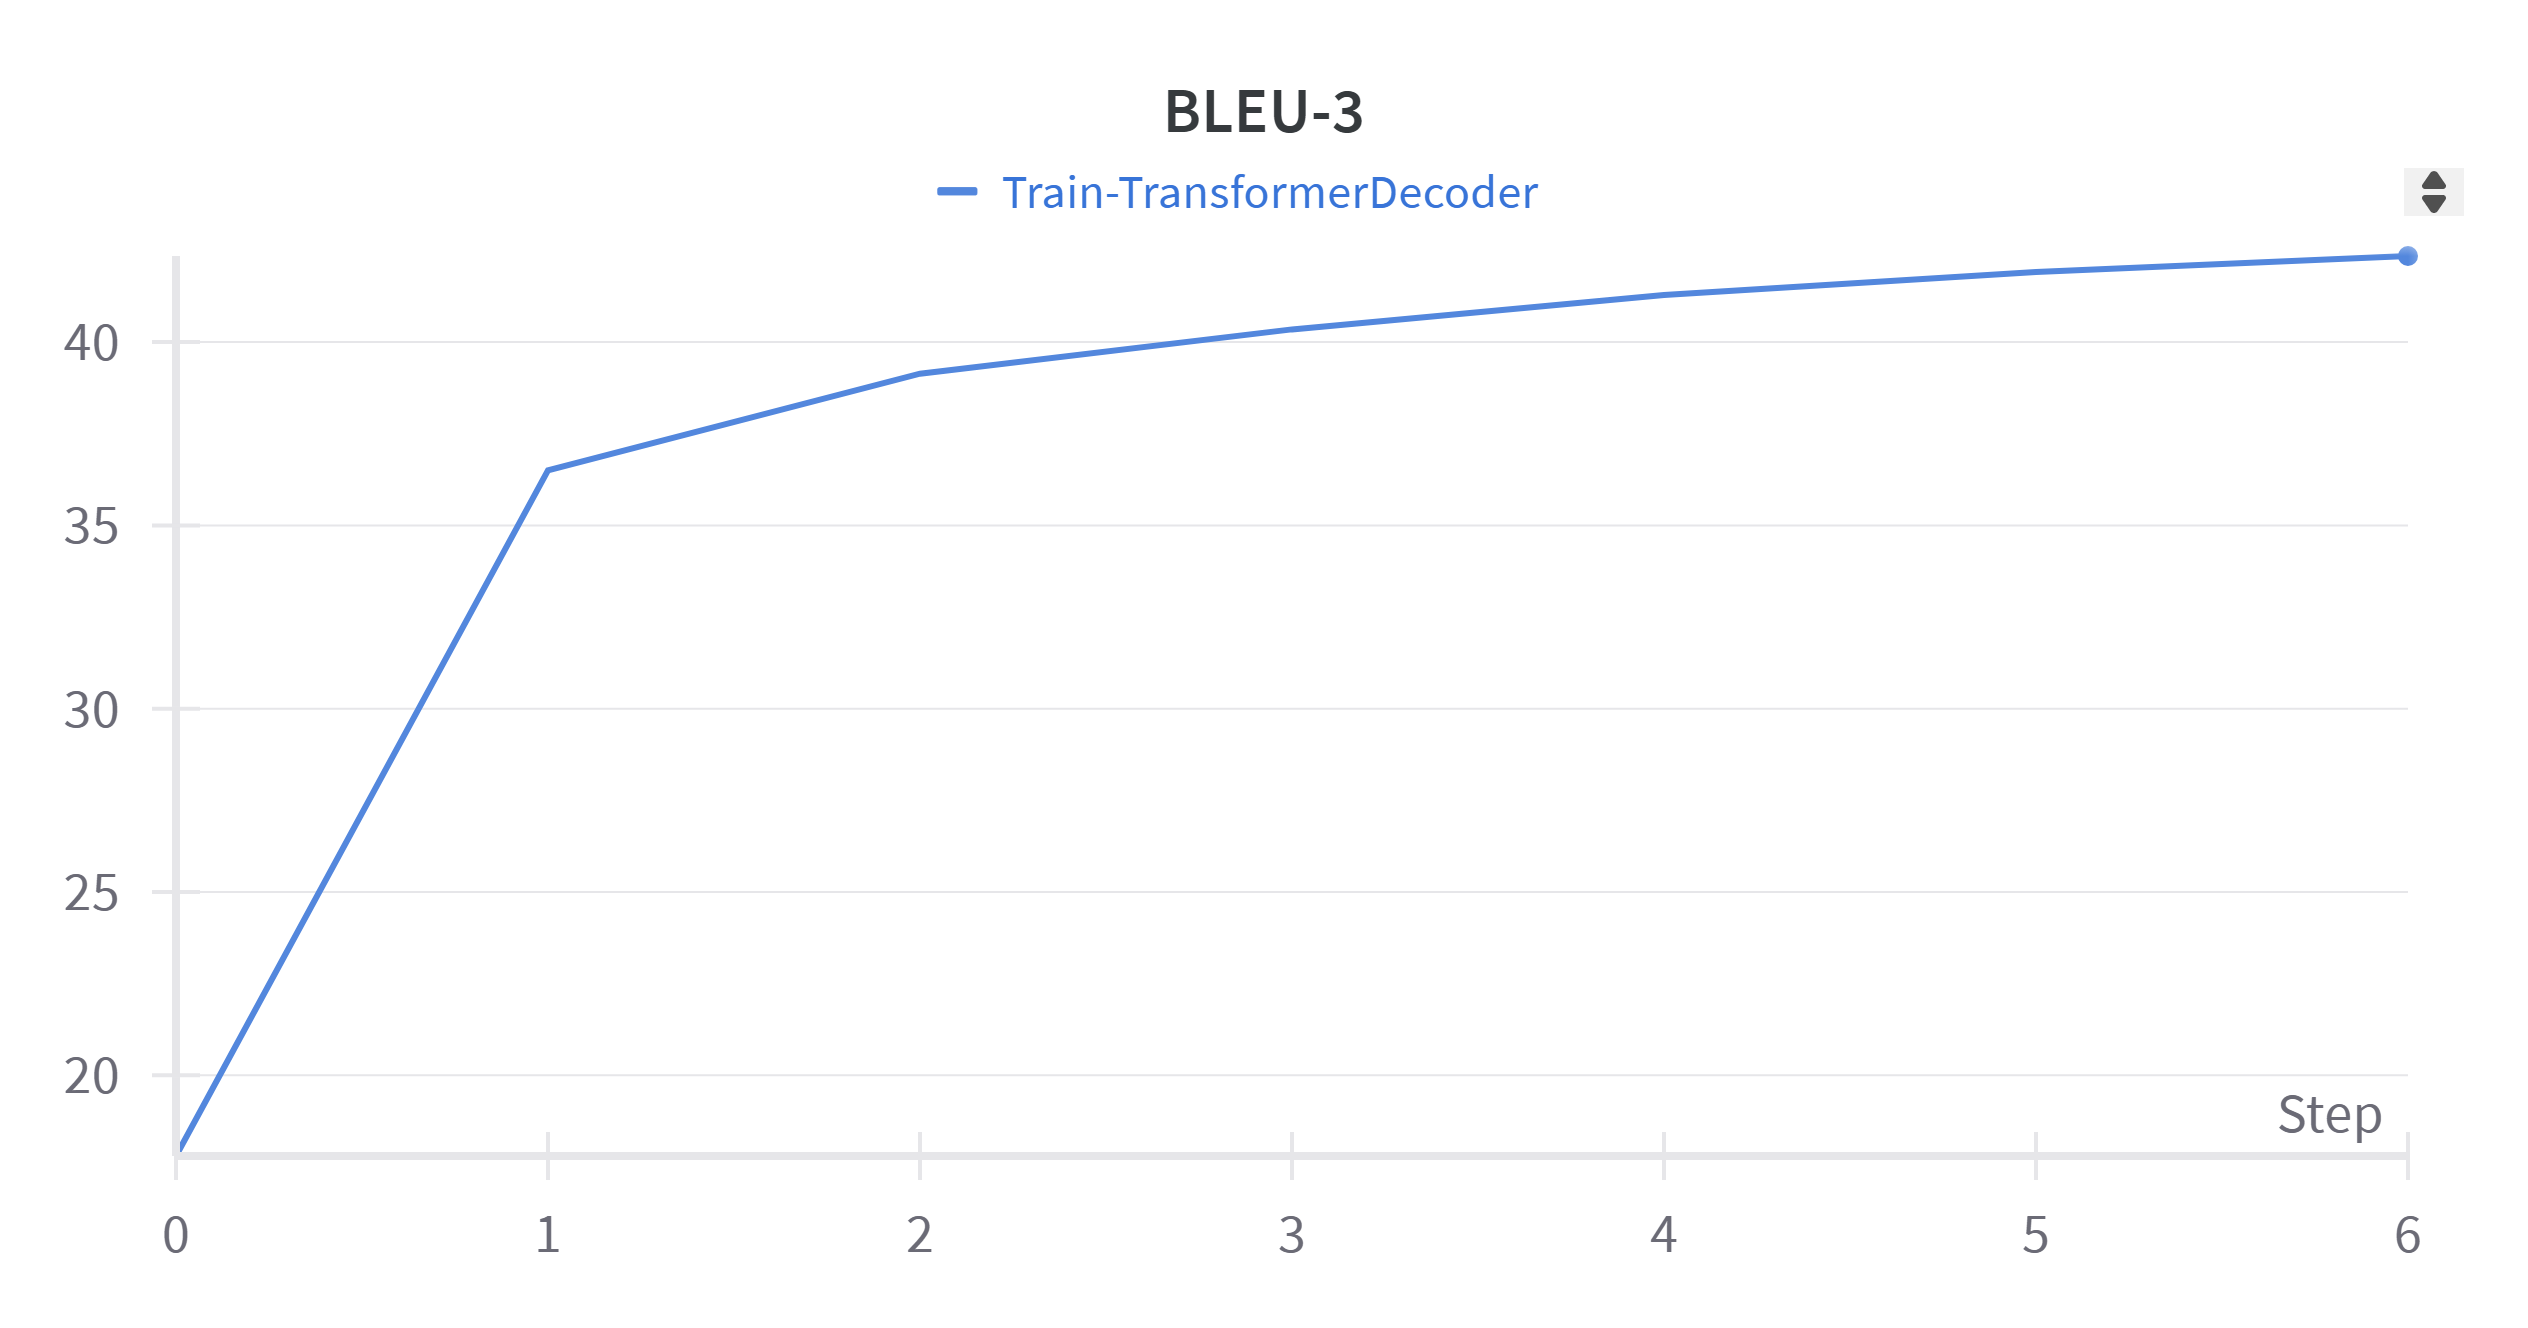
\includegraphics[width=\linewidth]{./wb-post-bleu3.png}
    \caption{BLEU-3}
    \label{fig:train_bleu_wo_attention}
  \end{subfigure}
  \hfill
  \begin{subfigure}[b]{0.49\textwidth}
    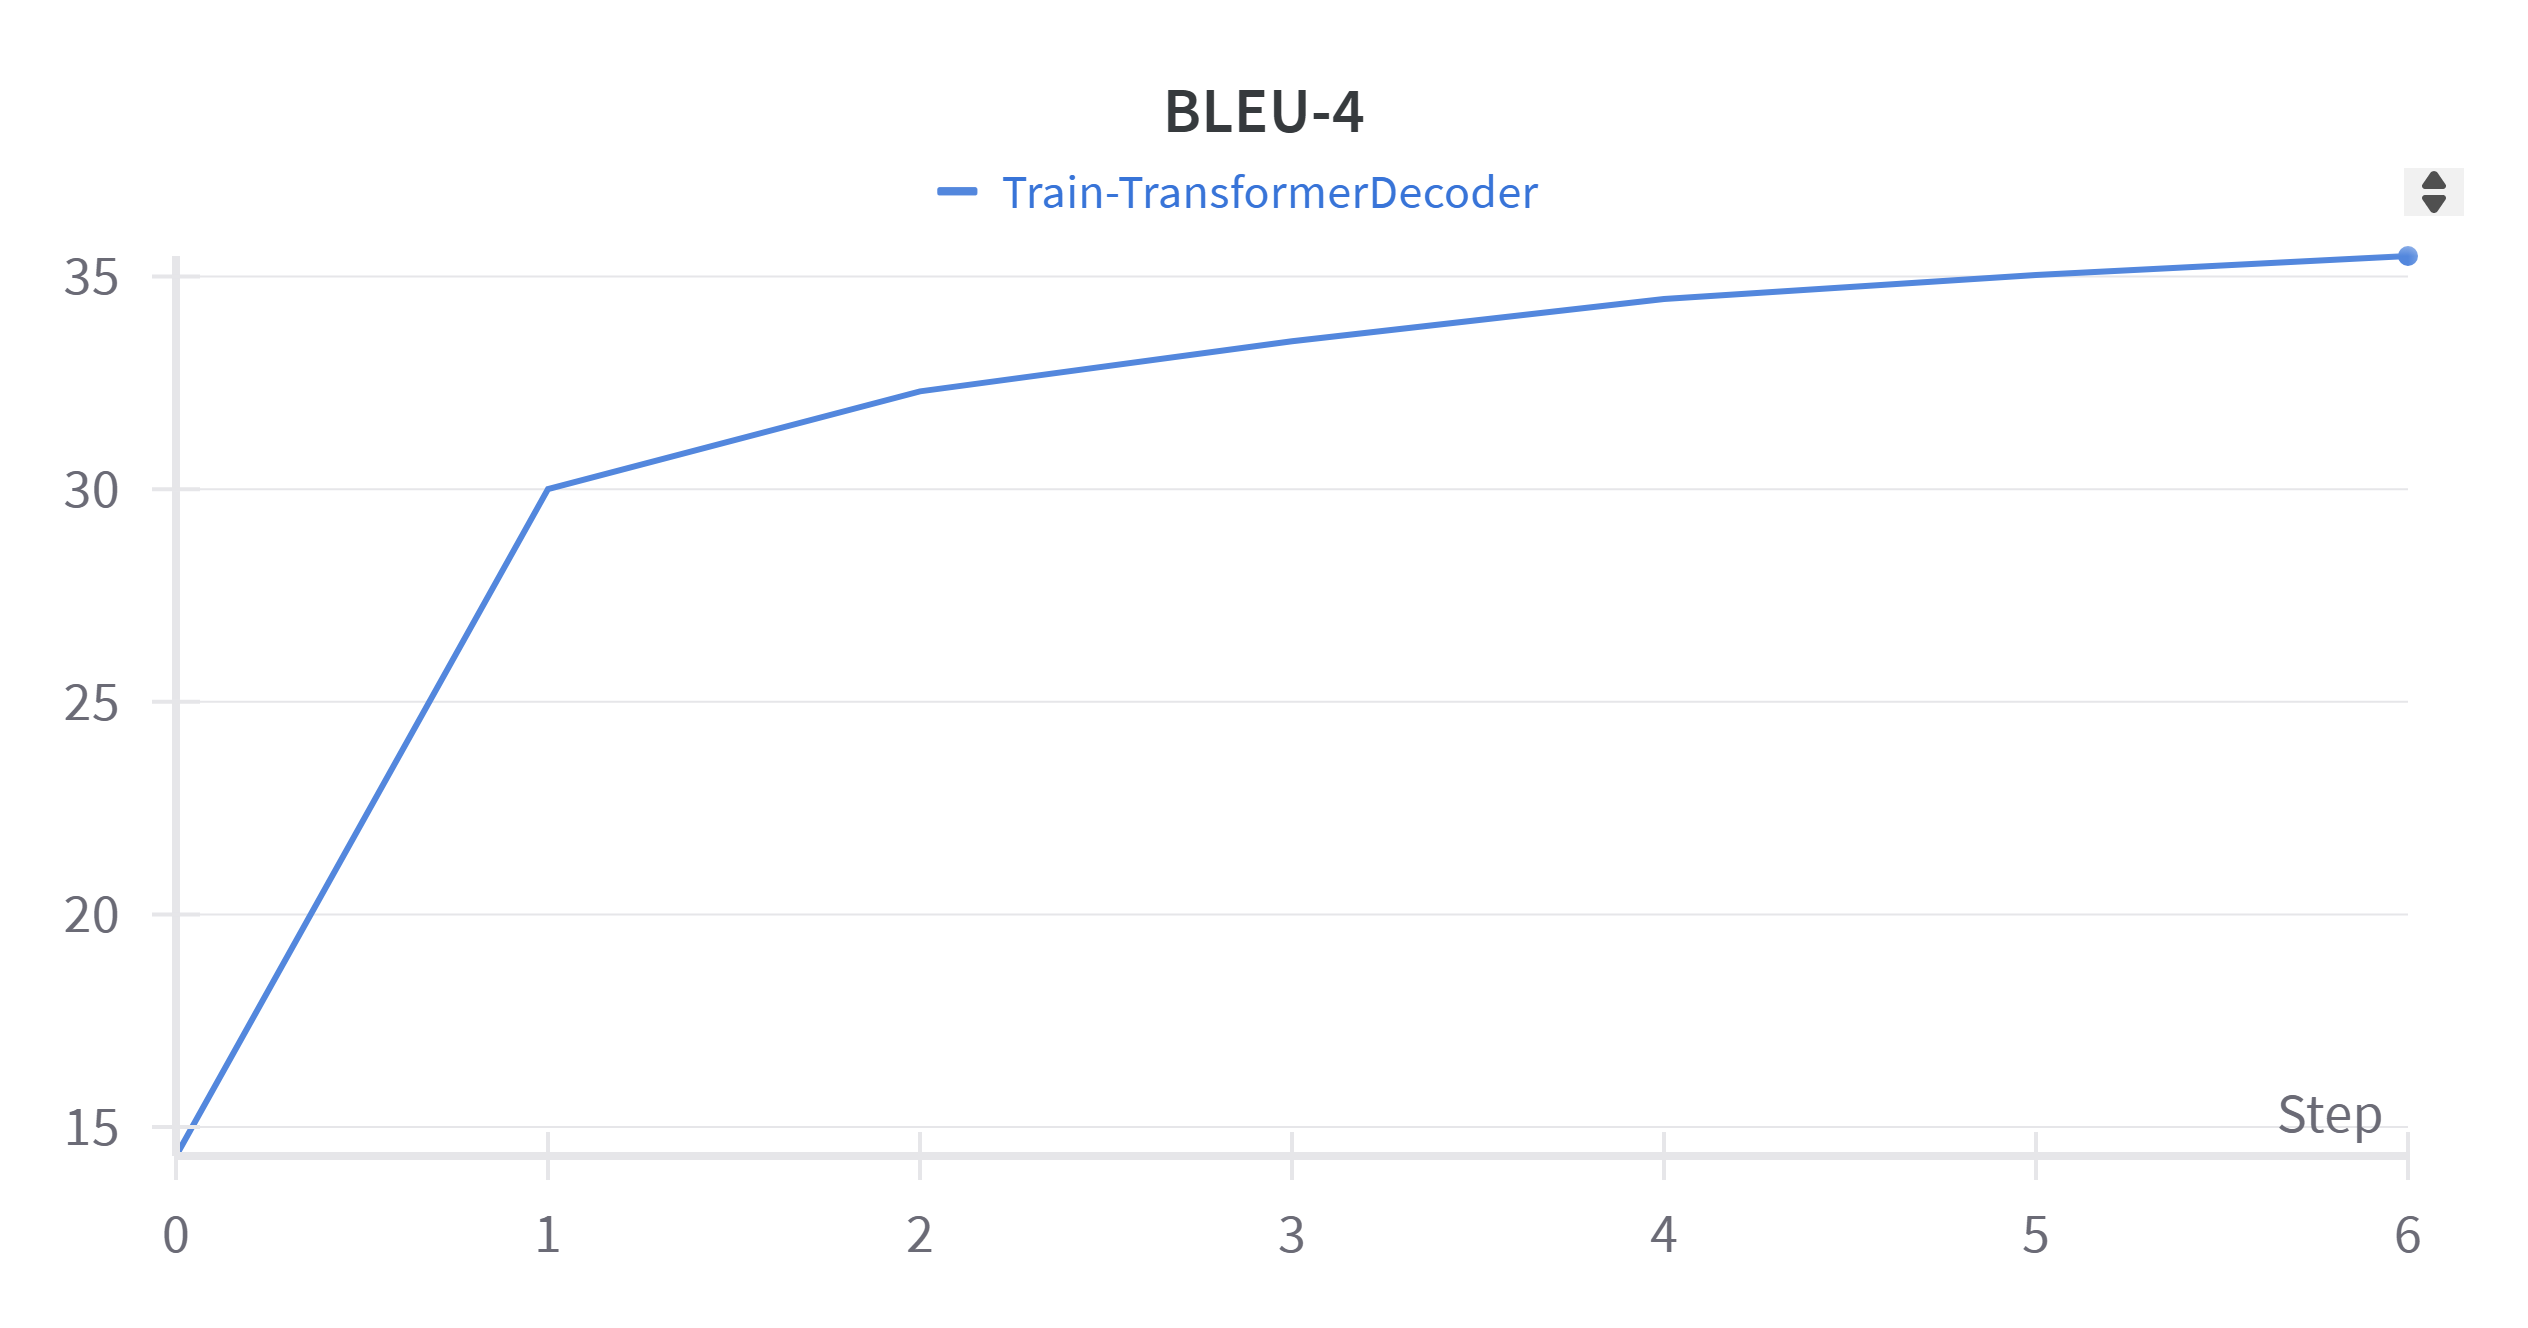
\includegraphics[width=\linewidth]{./wb-post-bleu4.png}
    \caption{BLEU-4}
    \label{fig:train_bleu_wo_attention}
  \end{subfigure}
  \caption{Wandb Training BLEU Score for Model with Post-layer Normalization}
  \label{fig:overall}
\end{figure}

\begin{figure}[H]
  \centering
  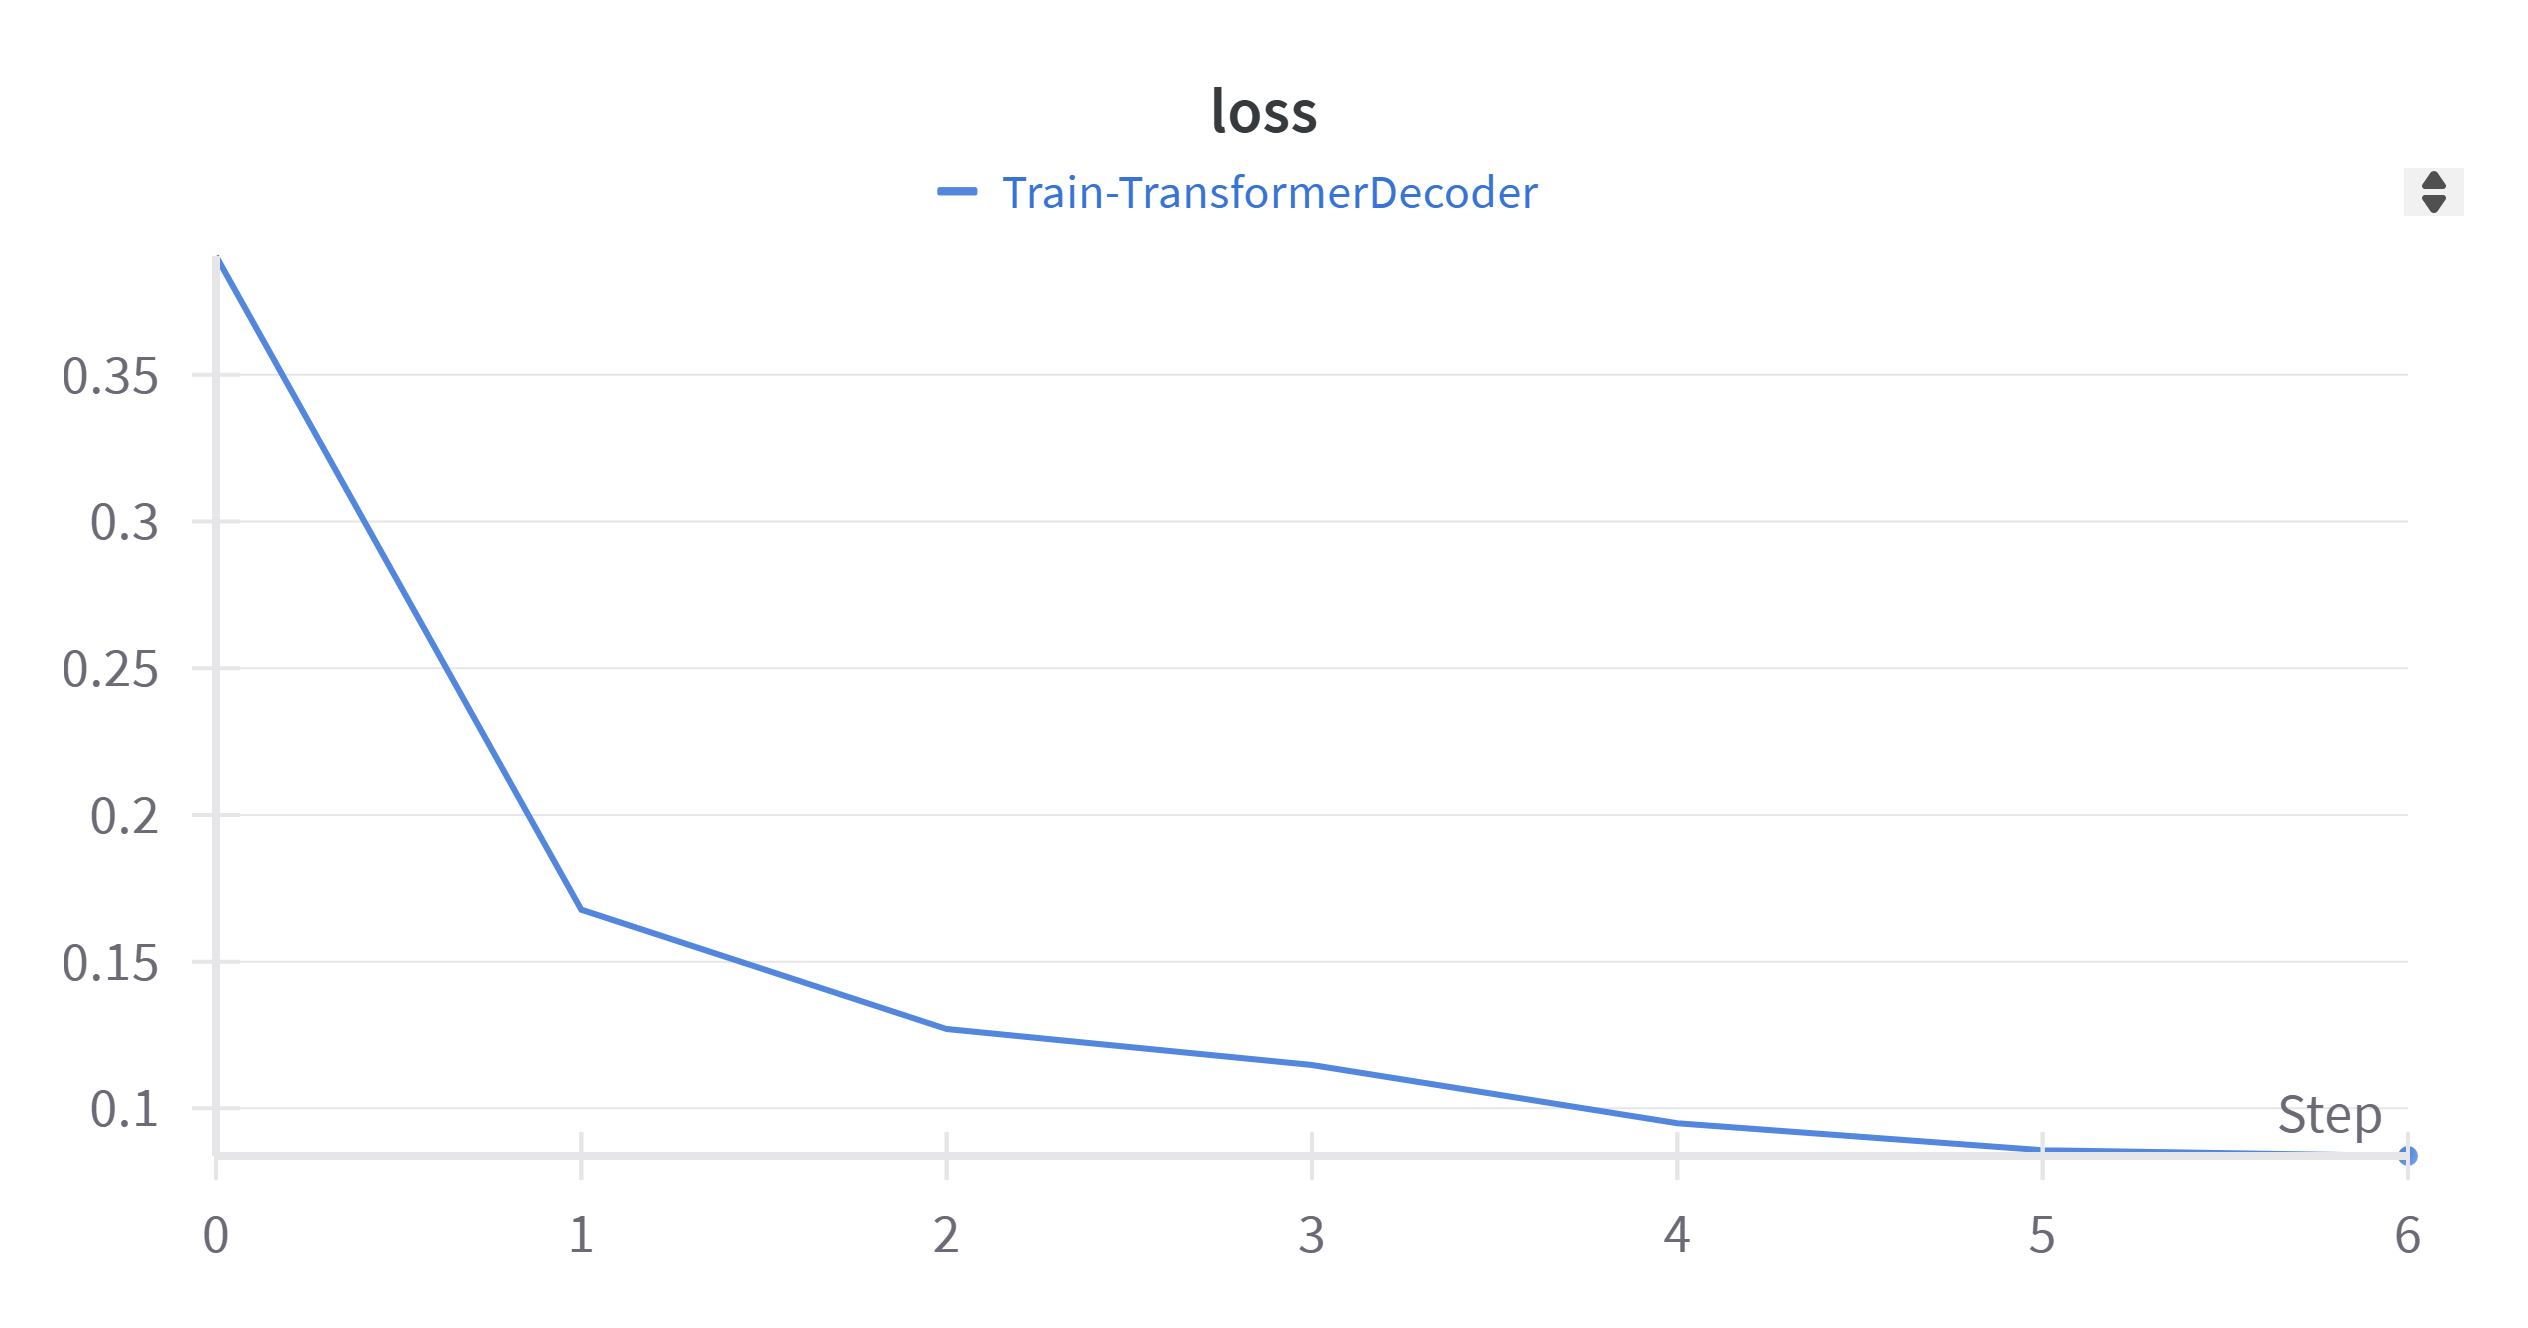
\includegraphics[width=0.5\linewidth]{./wb-post-loss.png}
  \caption{Wandb Training Loss for Model with Post-layer Normalization}
  \label{fig:train_loss_wo_attention}
\end{figure}

\begin{small}
\begin{verbatim}
  [Device:cuda] Epoch 1 Training ====
  [Device:cuda] Epoch 1 Validation ====
  Epoch 1: loss=0.3904670826544843, BLEU-4: 14.3199 BLEU-3: 17.7970, time=00:02:00
  [Device:cuda] Epoch 2 Training ====
  [Device:cuda] Epoch 2 Validation ====
  Epoch 2: loss=0.16770178072095168, BLEU-4: 30.0038 BLEU-3: 36.5013, time=00:04:04
  [Device:cuda] Epoch 3 Training ====
  [Device:cuda] Epoch 3 Validation ====
  Epoch 3: loss=0.1270381319860724, BLEU-4: 32.2994 BLEU-3: 39.1376, time=00:06:08
  [Device:cuda] Epoch 4 Training ====
  [Device:cuda] Epoch 4 Validation ====
  Epoch 4: loss=0.11475944897417063, BLEU-4: 33.4799 BLEU-3: 40.3467, time=00:08:11
  [Device:cuda] Epoch 5 Training ====
  [Device:cuda] Epoch 5 Validation ====
  Epoch 5: loss=0.09493687158571713, BLEU-4: 34.4729 BLEU-3: 41.2821, time=00:10:12
  [Device:cuda] Epoch 6 Training ====
  [Device:cuda] Epoch 6 Validation ====
  Epoch 6: loss=0.08575064966061739, BLEU-4: 35.0350 BLEU-3: 41.9148, time=00:12:15
  [Device:cuda] Epoch 7 Training ====
  [Device:cuda] Epoch 7 Validation ====
  Epoch 7: loss=0.0837674455684227, BLEU-4: 35.4824 BLEU-3: 42.3487, time=00:14:18
  Finished 7 epochs
\end{verbatim}
\end{small}


\subsection{Test Set BLEU Score}
This section lists the test set BLEU score reported on the test set for each model in table \ref{tab:bleu}.
\begin{table}[h]
\centering
\begin{tabular}{lcc} \toprule
Model                          & BLEU-4 &  BLEU-3 \\ \midrule
Model Pre-layer Normalization  & 40.9185 & 47.9510    \\
Model Post-layer Normalization & 29.6935 & 34.8660    \\
\bottomrule
\end{tabular}
\caption{The BLEU score reported on the test set for each model.}
\label{tab:bleu}
\end{table}

\newpage
\section{Translation Analysis}

\subsection{Translations}

\subsubsection{Transformer Model (Pre-Layer Norm)}
'<s> trudeau and <unk> are binding on the subject of the year </s>'\newline
'<s> a member of parliament is not surprised by his colleagues </s>'\newline
'<s> <unk> is telling his independence in exactly what he said </s>'\newline
'<s> the tories will promise their parents and your parent will be meeting your favourite tv </s>'\newline
'<s> trudeau visit to ottawa </s>'\newline
'<s> canada suffers from a crisis of productivity said that the government is doing nothing </s>'\newline
'<s> the federal government announces that canada will begin with seconds with seconds <unk> </s>'\newline
'<s> all the tory members pulled off the streets have to do that </s>'

\subsubsection{T5 MT}
"Trudeau and Colbert have a relationship around the status sharing of gars that were cool for 10 years"\newline
"A colleague in the world is not able to convince his colleagues to do what he wants"\newline
"Jagmeet Singh affirme his independence in doing exactly what Pierre Poilievre said to do"\newline
"The conservators say they are elus, your parents will agree, your television emission will not be annulled and McDonald’s will be ramening pizza"\newline
"Trudeau makes a surprise visit to Ottawa"\newline
"Canada suffers from a productivite crisis, affirming that the government does nothing"\newline
"The federal government announced that Canada would begin to swell with 15 secondes of incontournable publicities"\newline
"All that the Liberals had to interfere with Canadians in these last years"

\subsubsection{ChatGPT4o}
"Trudeau and Colbert bond over their shared status as guys who were cool ten years ago."\newline
"A colleague that everyone dislikes is surprised that he cannot convince his colleagues to do what he wants."\newline
"Jagmeet Singh asserts his independence by doing exactly what Pierre Poilievre told him to do."\newline
"The Conservatives promise that if they are elected, your parents will get back together, your favorite TV show will not be canceled, and McDonald’s will bring back pizza."\newline
"Trudeau makes a surprise visit to Ottawa."\newline
"Canada is suffering from a productivity crisis, claiming that the government is doing nothing."\newline
"The federal government announces that 'O Canada' will now start with 15 seconds of unskippable ads."\newline
"Everything that freedom-loving Conservatives have banned Canadians from doing in recent years."\newline


\subsection{Discussion}
{\it 
\begin{enumerate}
  \item My Transformer Model (Pre-Layer Norm) performs poorly compared to the other models. It doesn't translate sentences accurately and has many <unk> tokens. T5 MT is better, but sentences are not very natural. ChatGPT4o has the best translation, sentences are fluent.
  \item Training data quality, limited vocabulary size could affect the quality of the model's translations.
  \item Sentence translated better: '<s> trudeau visit to ottawa </s>'. Sentence translated worse: '<s> the tories will promise their parents and your parent will be meeting your favourite tv </s>'
        My Transformer Model (Pre-Layer Norm) is better at translating short, straightforward sentences, and not good at sentences with heavy context.
  \item The pattern persists on T5 MT, which is better, but still loses some contextual information when translating long, conplex sentences. The pattern does not persist on ChatGPT4o.
        This could be because of ChatGPT4o’s architecture, or its training on high-quality and diverse dataset, that enables it to have a better contextual understanding and fluency.
\end{enumerate}
}

\end{document}
